% ====================================================================
% Section: Proposed Methodology (Revised)
% ====================================================================
\section{Methodology}\label{sec:methodology}

This section details the methodology employed to design, implement, and evaluate the proposed adaptive IoT defense system. The framework is architected as a multi-stage, closed-loop process that synergizes predictive modeling with autonomous decision-making to create a proactive security posture. Section \ref{subsec:framework_architecture} provides a high-level overview of this architecture. Section \ref{subsec:data_source} describes the real-world dataset and preprocessing pipeline that form the empirical foundation of the system. The subsequent sections detail the design of the proactive attack prediction module (Section \ref{subsec:lstm_module}), the reinforcement learning environment (Section \ref{subsec:rl_environment}), and the training and benchmarking of the DRL defense agents (Section \ref{subsec:drl_training}).

% --- Subsection 3.1 ---
\subsection{Framework Architecture Overview}\label{subsec:framework_architecture}
The proposed framework is designed to transition IoT security from a reactive to a proactive paradigm. This is achieved through the architecture illustrated in Figure \ref{fig:framework_overview}, which can be understood through three primary stages.

\begin{figure}[h!]
    \centering
    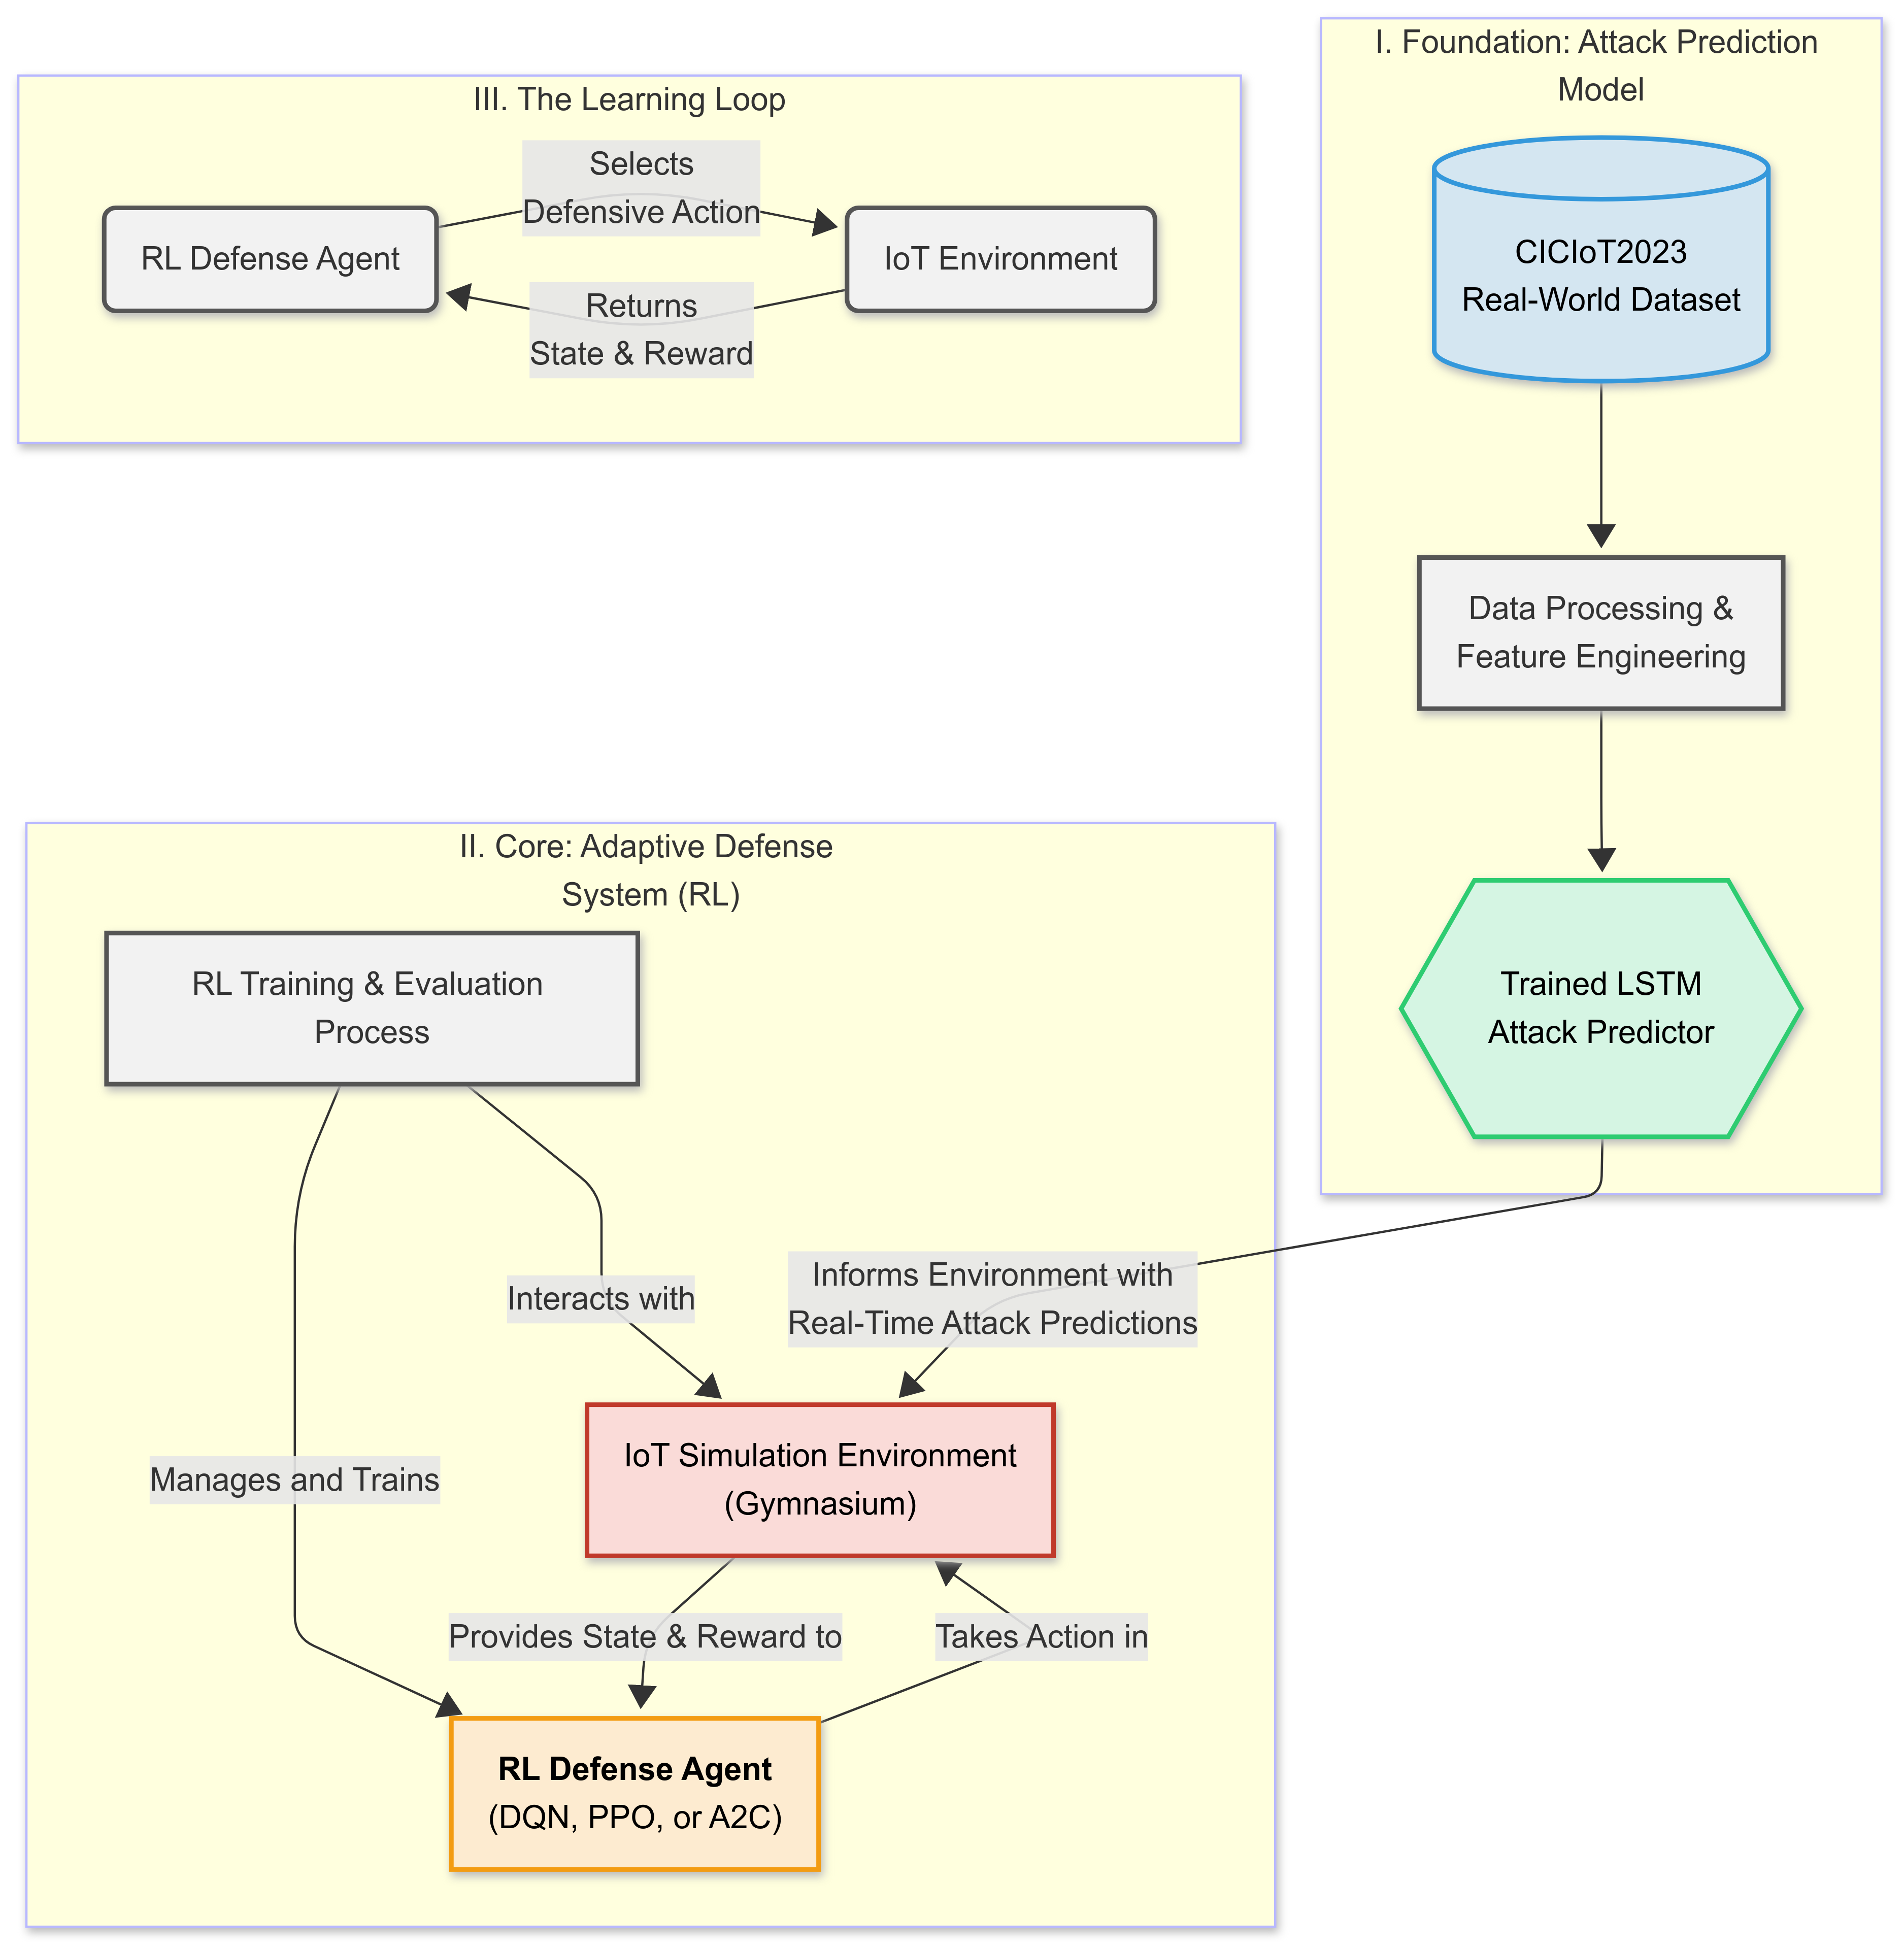
\includegraphics[width=0.85\textwidth]{figs/iot_rl_defense_system_diagram_mermaid.png}
    \caption{High-Level Architecture of the Proactive-Adaptive Defense System.}
    \label{fig:framework_overview}
\end{figure}

The three stages are:
\begin{enumerate}
    \item \textbf{Stage I: Predictive Foundation.} In this initial, offline stage, a Long Short-Term Memory (LSTM) based neural network is trained on a comprehensive, real-world IoT dataset. The objective is to develop a robust predictive model capable of identifying temporal patterns in network traffic that are indicative of imminent or ongoing cyberattacks. This pre-trained model serves as the system's "intelligence core," providing proactive threat assessments.
    
    \item \textbf{Stage II: Core Adaptive Defense System.} The second stage involves the primary training process for the defense agent. A DRL agent is trained within a custom-built simulation environment that models an IoT network. Crucially, this environment is informed by the predictions of the LSTM model from Stage I, which are integrated directly into the agent's observations.
    
    \item \textbf{Stage III: The Learning Loop.} This stage represents the fundamental reinforcement learning cycle that governs the adaptive defense system in Stage II. At each step of the simulation, the RL agent selects a defensive action, which is applied to the IoT environment. The environment, in turn, returns a new state and a corresponding reward signal. This continuous feedback loop is the mechanism through which the agent learns an optimal defense policy via trial and error.
\end{enumerate}
This decoupled architecture allows the system to ground its understanding of threats in real-world data (Stage I) while learning to apply that understanding to execute effective, autonomous defensive maneuvers through a formal learning process (Stages II and III).

% --- Subsection 3.2 ---
\subsection{Data Source and Preprocessing}\label{subsec:data_source}
The empirical validity of any AI-driven security system is fundamentally dependent on the quality and realism of its training data. This research utilizes the \textbf{CICIoT2023 dataset}, a contemporary and extensive resource for IoT security research \cite{Neto2023}.

\subsubsection{The CICIoT2023 Dataset}\label{subsubsec:dataset_desc}
The CICIoT2023 dataset was developed by the Canadian Institute for Cybersecurity (CIC) to address the need for a realistic benchmark reflecting modern IoT network traffic. Its key characteristics make it uniquely suited for this work:
\begin{itemize}
    \item \textbf{Realistic Testbed:} The data was captured from a physical topology of 105 real IoT devices, including smart cameras, speakers, sensors, and hubs \cite{Neto2023}.
    \item \textbf{Comprehensive Attack Coverage:} It contains benign traffic alongside labeled data for 33 distinct attack types, which are grouped into seven major categories: DDoS, DoS, Reconnaissance, Web-based, Brute Force, Spoofing, and Mirai variants \cite{Neto2023}.
    \item \textbf{Modern Attack Vectors:} A key feature of the dataset is that attacks were executed \textit{by} other compromised IoT devices within the testbed, simulating realistic botnet and device-to-device attack scenarios \cite{Neto2023}.
\end{itemize}

%\subsubsection{Data Preprocessing Pipeline}\label{subsubsec:preprocessing}
%To prepare the dataset for model training, a multi-step preprocessing pipeline was implemented. The raw network flow data, provided in CSV format, undergoes the following transformations:
%\begin{enumerate}
%    \item \textbf{Data Cleaning:} Rows with missing or infinite values are removed to ensure data integrity.
%    \item \textbf{Feature Scaling:} All numerical features are standardized using a `StandardScaler`. This process removes the mean and scales the data to unit variance, which is critical for the stable training of neural networks.
%    \item \textbf{Label Encoding:} The categorical attack labels are converted into a numerical format using a `LabelEncoder`.
%    \item \textbf{Data Splitting:} The dataset is divided into training (70\%), validation (15\%), and test (15\%) sets to ensure robust model evaluation and prevent overfitting.
%    \item \textbf{Sequence Generation:} For the LSTM model, the time-series data is transformed into sequences of a fixed length. Each sequence consists of a series of consecutive network flow feature vectors, with the label corresponding to the final time step in the sequence.
%\end{enumerate}
%The scaler and label encoder from this process are saved as artifacts to ensure consistent data transformation during both training and inference.

% --- Subsection 3.3 ---
\subsection{Proactive Attack Prediction Module}\label{subsec:lstm_module}
The proactive core of the framework is the attack prediction module, which is implemented as a Long Short-Term Memory (LSTM) network. LSTMs are a type of Recurrent Neural Network (RNN) specifically designed to learn long-term dependencies in sequential data, making them highly effective for time-series analysis of network traffic \cite{Hochreiter1997}.

\subsubsection{LSTM Model Architecture}
The attack prediction model consists of the following layers:
\begin{itemize}
    \item An \textbf{LSTM layer} that processes the input sequences of network features to capture temporal patterns.
    \item A \textbf{Dropout layer} for regularization to prevent overfitting.
    \item A series of \textbf{Fully Connected (Dense) layers} with ReLU activation functions to process the output from the LSTM layer.
    \item A final \textbf{Softmax output layer} that produces a probability distribution over all possible attack classes (including benign), representing the model's prediction.
\end{itemize}
The model is trained using the Adam optimizer and the Cross-Entropy Loss function, which are standard for multi-class classification tasks. The training process aims to minimize this loss, thereby learning an accurate mapping from a sequence of network data to a specific attack label.

% --- Subsection 3.4 ---
\subsection{Reinforcement Learning Environment Design}\label{subsec:rl_environment}
To train the DRL agents, a custom simulation environment was developed using the Gymnasium toolkit. This environment models the MDP described in Section \ref{subsubsec:mdp} and serves as the interactive training ground for the defense agents. Its core components are the state space, action space, and reward function.

\subsubsection{State and Action Spaces}
The environment is defined by a `Dict` observation space to provide the agent with a rich, multi-faceted view of the network's status.
\begin{itemize}
    \item \textbf{State Space ($S$):} The observation given to the agent at each timestep is a dictionary containing:
    \begin{itemize}
        \item \texttt{current\_state}: A vector of real-time network telemetry features.
        \item \texttt{state\_history}: A matrix containing a history of the last $N$ network states, allowing the agent to perceive temporal trends.
        \item \texttt{action\_history}: A vector of the last $M$ actions taken by the agent, providing it with self-awareness of its recent behavior.
        \item \texttt{attack\_prediction}: A vector of probabilities from the pre-trained LSTM model, representing the proactive assessment of the current threat level. This is the key link between the predictive and adaptive stages of the framework.
    \end{itemize}
    \item \textbf{Action Space ($A$):} The agent can select one of four discrete defensive actions:
    \begin{enumerate}
        \item \textbf{Monitor:} Take no action and continue observing.
        \item \textbf{Rate-Limit:} Restrict the traffic flow from suspicious sources.
        \item \textbf{Block IP:} Completely block traffic from identified malicious IPs.
        \item \textbf{Shutdown Service:} Temporarily disable a non-essential service under severe attack.
    \end{enumerate}
\end{itemize}

\subsubsection{Reward Function}
The design of the reward function is critical for guiding the agent toward the desired security posture. The function is engineered to balance threat mitigation with operational continuity. The composite reward at each timestep $t$, denoted $R_t$, is calculated as the sum of a prediction-based reward ($R_{pred}$) and an action-based reward ($R_{action}$):
$$ R_t = R_{pred} + R_{action} $$
Let $y_t \in \{0, 1\}$ be the true state of the network at timestep $t$ (where $1$ signifies an attack and $0$ signifies benign traffic), let $\hat{y}_t \in \{0, 1\}$ be the LSTM model's prediction, and let $\rho_t$ be the predicted risk score. The components are defined as follows:

\begin{itemize}
    \item \textbf{Prediction Reward ($R_{pred}$):} This component provides feedback based on the correctness of the LSTM's threat assessment. The reward is scaled by the model's confidence ($\rho_t$):
    \begin{equation}
    R_{pred} = 
    \begin{cases} 
        +10 \cdot \rho_t & \text{if } y_t=1 \text{ and } \hat{y}_t=1 \text{ (True Positive)} \\
        +5.0 & \text{if } y_t=0 \text{ and } \hat{y}_t=0 \text{ (True Negative)} \\
        -15 \cdot \rho_t & \text{if } y_t=1 \text{ and } \hat{y}_t=0 \text{ (False Negative)} \\
        -5 \cdot (1 - \rho_t) & \text{if } y_t=0 \text{ and } \hat{y}_t=1 \text{ (False Positive)}
    \end{cases}
    \end{equation}

    \item \textbf{Action Reward ($R_{action}$):} This component evaluates the suitability of the agent's action $a_t$ given the true state of the network. Actions are rewarded for effective mitigation during an attack and penalized for unnecessary disruption during benign traffic. Let $E(a_t)$ be an action's effectiveness bonus and $C(a_t)$ be its disruption cost, defined as:
    \begin{itemize}
        \item Action Effectiveness $E(a_t)$: Bonus values of $\{0.8, 0.9, 0.7, 0.6\}$ for actions \{`monitor`, `rate-limit`, `block IP`, `shutdown service`\}, respectively.
        \item Action Cost $C(a_t)$: Penalty values of $\{0.0, -1.0, -2.0, -3.0\}$ for the same actions.
    \end{itemize}
    The action reward is then:
    \begin{equation}
    R_{action} = 
    \begin{cases} 
        +5 \cdot E(a_t) & \text{if } y_t=1 \text{ (Attack ongoing)} \\
        C(a_t) & \text{if } y_t=0 \text{ (Benign traffic)}
    \end{cases}
    \end{equation}
\end{itemize}
This composite structure incentivizes the agent to learn a nuanced policy that trusts the predictor but also considers the operational impact of its actions, thereby balancing security with service continuity.

% --- Subsection 3.5 ---
\subsection{DRL Agent Training and Benchmarking}\label{subsec:drl_training}
The final component of the methodology is the training and evaluation of the DRL defense agents. To ensure robust and reproducible results, this work leverages the Stable Baselines3 library, a standard for high-quality DRL algorithm implementations.

\paragraph{Algorithm Selection}
Three prominent DRL algorithms were chosen to benchmark performance across different learning paradigms:
\begin{enumerate}
    \item \textbf{Deep Q-Network (DQN):} A classic value-based, off-policy algorithm that excels in discrete action spaces and serves as a strong baseline \cite{Mnih2015}.
    \item \textbf{Proximal Policy Optimization (PPO):} A state-of-the-art on-policy, actor-critic algorithm known for its stability and reliable performance \cite{Schulman2017}.
    \item \textbf{Advantage Actor-Critic (A2C):} A synchronous, on-policy actor-critic method that is often faster than PPO and provides another point of comparison \cite{Mnih2016}.
\end{enumerate}
All agents use a `MultiInputPolicy` architecture, which is specifically designed to process the `Dict` observation space from the custom IoT environment.